\section{Endpoint asymptotics at saddle mergers and nested horizontal potentials}\label{sec:horizontal}

Consider the model Hamiltonian $W(X)+Z^{2\alpha}$ on $\R^2$, where $\alpha\ge 2$ is an even integer and $W\in\R[X]$ is a real polynomial. At a nondegenerate maximum \(X_s\) of \(W\) the energy relative to its critical value has local form \(Z^{2\alpha}-\xi^2\), after a regular horizontal change of coordinate. The zero level has two incoming and two outgoing separatrices. The Hamiltonian linearization at \((X_s,0)\) is nonzero with square zero because \(W''(X_s)<0\) and the vertical second derivative vanishes. This is the nilpotent saddle at which the two families of ovals merge.

Away from critical values of $W$, each bounded connected component $I(E)$ of $\{X\in\R : W(X)<E\}$ defines a vertically symmetric Jordan domain $\Omega_I(E)=\{(X,Z): X\in I(E),\; |Z|<(E-W(X))^{1/(2\alpha)}\}$ bounded by a smooth regular oval. Integrating the $Z$-derivative of an odd monomial $Z^{2j+1}$ ($j\ge 0$) over $\Omega_I(E)$ yields twice the slice moment
\begin{equation}\label{eq:model-moment}
  F_{j,I}(E) := \int_{I(E)} (E-W(X))^{\gamma_j}\dd X, \qquad
  \gamma_j := \frac{2j+1}{2\alpha}, \qquad \nu_j := \gamma_j + \frac{1}{2}.
\end{equation}
Because $\alpha$ is even, $2j+1$ and $2j+1+\alpha$ are odd whereas $2\alpha$ is even; thus neither $\gamma_j$ nor $\nu_j$ is ever an integer. On any open energy interval of regular ovals, $F_{j,I}(E)$ is real-analytic in $E$.

As in the double-well example of Section~\ref{sec:intro}, each of the \(q\) minima starts a family, and each of the \(q-1\) distinct positive saddle levels ends two families and starts one enclosing family. This gives \(2q-1\) maximal annuli and \(4q-3\) finite ends. Equal heights can change the count. For \(W=T_3^2\) the three wells merge at height one, giving seven finite ends.

A regular energy bracket belongs to one specified family, and its collar is the union of the ovals in that bracket. Figure~\ref{fig:fold-geometry} illustrates the count for four wells.

\begin{figure}[htbp]
\centering
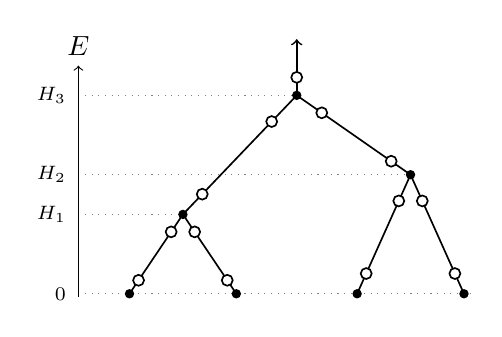
\begin{tikzpicture}[x=1.18cm,y=.84cm,
 endmark/.style={circle,draw,fill=white,inner sep=1.4pt}]
 \coordinate (a) at (0,0); \coordinate (b) at (1.15,0);
 \coordinate (c) at (2.45,0); \coordinate (d) at (3.60,0);
 \coordinate (u) at (.575,1.20); \coordinate (v) at (3.025,1.80);
 \coordinate (w) at (1.80,3.00);
 \draw[dotted,gray] (-.55,0) -- (3.70,0);
 \draw[dotted,gray] (-.55,1.20) -- (u);
 \draw[dotted,gray] (-.55,1.80) -- (v);
 \draw[dotted,gray] (-.55,3.00) -- (w);
 \foreach \start/\finish in {a/u,b/u,c/v,d/v,u/w,v/w}{
   \draw[semithick] (\start) -- node[endmark,pos=.17] {}
     node[endmark,pos=.78] {} (\finish);
 }
 \draw[semithick,->] (w) -- node[endmark,pos=.32] {} (1.80,3.85);
 \foreach \pt in {a,b,c,d,u,v,w}{\fill (\pt) circle[radius=1.7pt];}
 \draw[->] (-.55,-.05) -- (-.55,3.45) node[above] {\(E\)};
 \node[left,font=\scriptsize] at (-.58,0) {\(0\)};
 \node[left,font=\scriptsize] at (-.58,1.20) {\(H_1\)};
 \node[left,font=\scriptsize] at (-.58,1.80) {\(H_2\)};
 \node[left,font=\scriptsize] at (-.58,3.00) {\(H_3\)};
\end{tikzpicture}
\caption{Schematic of three saddle mergers for four wells at distinct heights \(H_1<H_2<H_3\). Edges represent maximal period annuli. Hollow circles mark the two finite ends of each bounded edge and the single finite end of the outer edge, thirteen in all. The lower bound for crossings near each marked end depends on its type and on the available modes in \eqref{eq:Bqalpha}.}
\label{fig:fold-geometry}
\end{figure}


At a merger the outer limiting interval is the union of the two inner intervals up to the saddle point. At a saddle height \(H_*\), each coefficient of \((E-H_*)^\ell\) for an integer \(0\le\ell<\nu_j\) in the slice moment \(F_{j,I}\) is a convergent integral over that interval. The two incoming sets of cancellations thus suffice for all three one-sided families. For nilpotent double loops, Yang, Yu and Han obtain a constant-term addition law \cite[(3.17)]{YangYuHan2019} and higher coefficients for centrally symmetric cuspidal loops under recursive analytic hypotheses \cite[Theorem~3.1]{YangYuHan2021}. For a hyperbolic saddle Xu, Yang and Han record the regular addition law \cite[(1.5)--(1.6)]{XuYangHan2024}, citing \cite{HanYangLi2023}. Here the slice integral gives every coefficient preceding its first fractional power, together with the one-sided signs needed to count crossings.

\FloatBarrier
\begin{lemma}[Local expansions and intrinsic signs at extrema]\label{lem:saddle-singular}
Fix $j\ge 0$, write $\gamma=\gamma_j$, $\nu=\nu_j$, $k_j=\lfloor\nu\rfloor$, and let $v>0$ denote the energy distance $\lvert E-E_*\rvert$ to a Morse critical value $E_*$ of $W$.
\begin{enumerate}[label=(\alph*),nosep]
  \item At a nondegenerate local minimum of height $E_*=0$, $F_{j,I}(v)=c_0 v^\nu(1+O(v))$ as $v\downarrow 0$ with $c_0>0$.
  \item Suppose a nondegenerate maximum of height $E_*=H_*$ joins two bounded sublevel intervals into one and the two outer turning points at that height are simple. On each of the two incoming branches ($E=H_*-v$) and on the outgoing branch ($E=H_*+v$), one has as $v\downarrow 0$
  \begin{equation}\label{eq:local-saddle-jet}
    F_{j,I}(H_*\pm v) = \sum_{\ell=0}^{k_j} A_{\ell,I} (\pm v)^\ell + C_I v^\nu + o(v^\nu),
  \end{equation}
  where $\sgn C_I = (-1)^{k_j+1}$ on each incoming branch and $\sgn C_I = \sgn(\gamma-k_j)$ on the outgoing branch. Moreover, for every $0\le\ell\le k_j$, the outgoing signed-energy Taylor coefficient $A_{\ell,\mathrm{out}}$ equals the sum $A_{\ell,\mathrm{in},-}+A_{\ell,\mathrm{in},+}$ of the two incoming signed-energy Taylor coefficients.
\end{enumerate}
\end{lemma}

\begin{proof}
At a nondegenerate minimum, choose a local analytic Morse coordinate $w$ with $W(X)=w^2$ and $\dd X/\dd w = A_0(w)>0$. Rescaling $w=\sqrt{v}\,u$ gives $F_{j,I}(v)=v^\nu\int_{-1}^1 (1-u^2)^\gamma A_0(\sqrt{v}\,u)\dd u = A_0(0)\Bta(\tfrac{1}{2},\gamma+1)v^\nu(1+O(v))$, proving~(a).

Near a nondegenerate maximum $X_*$ with $W(X_*)=H_*$, choose an orientation-preserving analytic coordinate $w$ on $[-c,c]$ ($c>0$) such that $W(X)=H_*-w^2$ and $\dd X/\dd w = A(w)>0$. Apart from the saddle and neighborhoods of the simple outer turning points, $H_*-W(X)$ is bounded below by a positive constant on the remaining compact intervals. Taking $W$ itself as local coordinate near a simple outer turning point $X_{\mathrm{turn}}(E)$ shows that $\int (E-W)^\gamma (\dd X/\dd W)\dd W$ extends smoothly in $E$ across $E=H_*$. Thus all non-smoothness at $E=H_*$ comes from the local integral over $w\in[-c,c]$.

On the right incoming branch ($E=H_*-v$, $w\in[\sqrt{v},c]$; the left branch $w\in[-c,-\sqrt{v}]$ is identical with $A(-w)$), the local integral is $\int_{\sqrt{v}}^c (w^2-v)^\gamma A(w)\dd w$. Substituting $t=w^2-v$ gives
\[
  \frac{1}{2}\int_0^{c^2-v} t^\gamma (t+v)^{-1/2} A\bigl(\sqrt{t+v}\bigr)\dd t.
\]
Expand $A(\pm\sqrt{s})=A(0)\pm s^{1/2}B_1(s)+s B_2(s)$ with $B_1,B_2$ analytic near $s=0$. Differentiate $k_j+1$ times with respect to $v$:
\begin{itemize}[nosep]
  \item Boundary terms at the upper limit $c^2-v$ are smooth and $O(1)$ as $v\downarrow 0$.
  \item For the odd-coordinate piece $\pm(t+v)^{1/2}B_1(t+v)$, the singular factor $(t+v)^{-1/2}$ cancels $(t+v)^{1/2}$ identically, leaving the analytic function $\pm B_1(t+v)$ whose $(k_j+1)$-st $v$-derivative is bounded on $[0,c^2-v]$ and contributes $O(1)$.
  \item The even remainder $(t+v)^{-1/2}\cdot(t+v)B_2(t+v)=(t+v)^{1/2}B_2(t+v)$ has $(k_j+1)$-st $v$-derivative $O((t+v)^{-k_j-1/2})$, whose integral against $t^\gamma$ is $O(1)$ (for $k_j=0$ it integrates directly to $O(1)$, and for $k_j\ge 1$ scaling $t=vz$ near $0$ gives $O(v^{\nu-k_j})+O(1)=O(1)$ since $\nu>k_j$).
  \item The principal $A(0)$ piece gives $\frac{1}{2}A(0)(-1)^{k_j+1}(\tfrac{1}{2})_{\overline{k_j+1}}\int_0^{c^2-v} t^\gamma(t+v)^{-k_j-3/2}\dd t$. Here \((a)_{\overline m}=\prod_{j=0}^{m-1}(a+j)\). Scaling $t=vz$ yields
  \[
    \frac{1}{2}A(0)(-1)^{k_j+1}\bigl(\tfrac{1}{2}\bigr)_{\overline{k_j+1}}\Bta\bigl(\gamma+1,\,k_j+\tfrac{1}{2}-\gamma\bigr)v^{\nu-k_j-1} + O(1),
  \]
  where the Beta integral converges since $\gamma>-1$ and $k_j+\frac{1}{2}-\gamma=k_j+1-\nu>0$.
\end{itemize}
Since $\nu-k_j-1\in(-1,0)$, integrating $k_j+1$ times from $0$ to $v$ divides by $(\nu)_{\underline{k_j+1}}=\nu(\nu-1)\cdots(\nu-k_j)>0$ (every factor is strictly positive because $k_j<\nu<k_j+1$) and produces~\eqref{eq:local-saddle-jet} on each incoming side with $\sgn C_{\mathrm{in}}=(-1)^{k_j+1}$.

On the outgoing branch ($E=H_*+v$), we integrate $(w^2+v)^\gamma A(w)$ over $[-c,c]$. The odd part of $A(w)$ cancels, leaving $\int_{-c}^c (w^2+v)^\gamma(A(0)+w^2 B_2(w^2))\dd w$. Differentiating $k_j+1$ times with respect to $v$ under the integral gives $(\gamma)_{\underline{k_j+1}}\int_{-c}^c (w^2+v)^{\gamma-k_j-1}(A(0)+O(w^2))\dd w$. Rescaling $w=\sqrt{v}\,z$, the $O(w^2)$ error is $O(1+v^{\nu-k_j})=O(1)$, while the $A(0)$ term gives $A(0)(\gamma)_{\underline{k_j+1}}\Bta(\tfrac{1}{2},k_j+\tfrac{1}{2}-\gamma)v^{\nu-k_j-1}+O(1)$ (convergent since $k_j+\frac{1}{2}-\gamma>0$). In $(\gamma)_{\underline{k_j+1}}=\gamma(\gamma-1)\cdots(\gamma-k_j)$, the first $k_j$ factors satisfy $\gamma-(k_j-1)=\nu-k_j+\frac{1}{2}>\frac{1}{2}>0$, so $\sgn(\gamma)_{\underline{k_j+1}}=\sgn(\gamma-k_j)$. Integrating $k_j+1$ times divides by $(\nu)_{\underline{k_j+1}}>0$, establishing $\sgn C_{\mathrm{out}}=\sgn(\gamma-k_j)$.

It remains to identify the regular coefficients on the three sides. Write \(\beta=\gamma-\ell\) for \(0\le\ell\le k_j\), so \(\beta>-1/2\). At a regular energy the first \(\ell\) signed-energy derivatives have integrands \((\gamma)_{\underline{\ell}}(E-W)^\beta\). Indeed, before each differentiation the power at a simple turning point is positive, so its boundary term vanishes, and the resulting power is locally integrable. To pass to \(E=H_*\), fix an interior cutoff \(X_0\) near each simple outer turning point on a monotone branch of \(W\). In \(u=E-W(X)\) that endpoint piece, omitting the constant factor, is
\[
  \int_0^{E-W(X_0)} u^\beta
     \left|(W^{-1})'(E-u)\right|\,\mathrm du .
\]
The inverse derivative is smooth and bounded on the chosen branch. The upper limit tends to a positive number, and \(\beta>-1\) gives convergence at \(u=0\). On the compact parts away from turning points and the saddle the integrands converge uniformly.

In the saddle chart alone, split at \(|w|=2\sqrt v\). On \(2\sqrt v\le |w|\le c\), the factors \(w^2\pm v\) are comparable to \(w^2\), so \(C|w|^{2\beta}\) is an integrable majorant. In the inner part put \(w=\sqrt v\,z\). Its absolute contribution is \(O(v^{\beta+1/2})=O(v^{\nu-\ell})\). The rescaled integral contains \((z^2+1)^\beta\) on \(|z|\le2\) above the saddle, or \((z^2-1)^\beta\) on \(1\le|z|\le2\) below, both integrable. Thus on each side
\[
 A_{\ell,I}=\frac{(\gamma)_{\underline{\ell}}}{\ell!}
      \int_{I(H_*)}(H_*-W(X))^{\gamma-\ell}\,\mathrm dX .
\]
The limiting outgoing interval is the union of the two incoming intervals up to the saddle point. Additivity of the displayed integrals gives the asserted identity for the signed-energy Taylor coefficients.
\end{proof}

Write $\pos{t}=\max(t,0)$. For integers $q\ge 2$, $\alpha\ge 2$ even, and $L\ge 1$, set $B_{q,\alpha}(0):=0$ and
\begin{equation}\label{eq:Bqalpha}
  \begin{gathered}
    b := \left\lfloor\frac{L-1+\alpha/2}{\alpha}\right\rfloor, \qquad
    c := \left\lfloor\frac{2(L-1)}{\alpha}\right\rfloor, \qquad
    J := L - 2(q-1)(b+1) - 1, \\
    B_{q,\alpha}(L) := q\pos{J} + 2(q-1)\pos{J-b} + (q-1)\pos{J-c}.
  \end{gathered}
\end{equation}

\begin{lemma}[Simultaneous endpoint brackets on a $q$-well cluster]\label{lem:endpoint-cluster}
Let $f\in\R[X]$ be a polynomial of degree $q\ge 2$ with $q$ simple real roots and $q-1$ critical points at which $f^2$ takes pairwise distinct positive values, and put $W=f^2$. For every even $\alpha\ge 2$ and every integer $L\ge 1$, there exists an odd rational polynomial $S\in\Q[Z]$ of degree at most $2L-1$ whose integrated derivative $\iint_{\Omega_I(E)} S'(Z)\dd X\dd Z$ has at least $\pos{J}$ regular energy brackets near each minimum, $\pos{J-b}$ on each incoming saddle branch and $\pos{J-c}$ on each outgoing branch, for a total of at least $B_{q,\alpha}(L)$. Their compact annular collars are pairwise disjoint in the $(X,Z)$-plane. On each bracket the moment has opposite endpoint signs and its energy derivative is bounded strictly away from zero.
\end{lemma}

\begin{proof}
If $J\le 0$ then $B_{q,\alpha}(L)=0$ and any rational $S$ suffices; assume $J\ge 1$. Consider $S(Z)=\sum_{j=0}^{L-1} a_j Z^{2j+1}$ with coefficient vector $a=(a_0,\dots,a_{L-1})\in\R^L$. Note that $\max_{0\le j<L}\lfloor\nu_j\rfloor=\lfloor\frac{L-1}{\alpha}+\frac{1}{2}\rfloor=b$. At each of the $q-1$ distinct saddle heights $H_*$ and on each of its two incoming branches, impose the $b+1$ homogeneous linear equations $\sum_{j:\,\ell<\nu_j} A_{\ell,I}^{(j)} a_j = 0$ ($0\le\ell\le b$), where $A_{\ell,I}^{(j)}$ is the signed-energy Taylor coefficient of $F_{j,I}$ from Lemma~\ref{lem:saddle-singular}(b). There are $2(q-1)(b+1)$ homogeneous linear equations on $\R^L$, so their joint real kernel $\mathcal N$ has dimension $n_0\ge L-2(q-1)(b+1)=J+1\ge 2$ without any independence assumption on the rows. By Lemma~\ref{lem:saddle-singular}(b), every $a\in\mathcal N$ also satisfies $\sum_{j:\,\ell<\nu_j} A_{\ell,\mathrm{out}}^{(j)} a_j=0$ ($0\le\ell\le b$) at every saddle.

Choose a row-echelon basis $v^{(0)},\dots,v^{(n_0-1)}$ of $\mathcal N$ ordered by strictly increasing first nonzero column indices $0\le p_0<p_1<\cdots<p_{n_0-1}\le L-1$, normalized to have $v^{(i)}_{p_i}=1$ and $v^{(i)}_j=0$ for $j<p_i$. Fix $i\in\{0,\dots,n_0-1\}$. Because every nonzero entry $v^{(i)}_j$ has $j\ge p_i$, for each integer $\ell<\nu_{p_i}$ we also have $\ell<\nu_j$, so all columns occurring in $v^{(i)}$ participate in row $\ell$ and cancel the $\ell$-th Taylor term exactly. Every uncanceled integer Taylor term has order $\ell>\nu_{p_i}$, and columns $j>p_i$ have fractional order $\nu_j>\nu_{p_i}$. Therefore, on every incoming and outgoing saddle branch $I$, the moment of $v^{(i)}$ has leading asymptotic $2 C_I^{(p_i)} v^{\nu_{p_i}}(1+o(1))$ as $v=|E-H_*|\downarrow 0$, with the intrinsic sign of column $p_i$ from Lemma~\ref{lem:saddle-singular}(b), while at each of the $q$ minima ($E=v\downarrow 0$) it has positive leading term $2c_{0,I}^{(p_i)} v^{\nu_{p_i}}(1+o(1))$.

To separate the leading orders of the saddle moments, fix an integer $A_0>L$, let $\rho\in(0,1)$, and form $a(\rho)=\sum_{i=0}^{n_0-1}(-1)^i\rho^{(A_0-p_i)^2} v^{(i)}$. Evaluate at the $n_0$ energy offsets $v_m=\rho^{2\alpha(A_0-p_m)}$ ($0\le m<n_0$). Since $\nu_{p_i}=\nu_0+p_i/\alpha$, the leading term of $v^{(i)}$ at $v_m$ has magnitude proportional to
\[
  \rho^{(A_0-p_i)^2 + 2\alpha(A_0-p_m)(\nu_0+p_i/\alpha)}
  = \rho^{2\alpha(A_0-p_m)\nu_0 + A_0^2 - p_m^2 + (p_i-p_m)^2}.
\]
Every $i\ne m$ carries an extra positive exponent $(p_i-p_m)^2\ge 1$ in $\rho$, and the remainder of the dominant column is \(o(1)\) relative to its leading term as \(v_m\downarrow0\). Hence for a single sufficiently small $\rho\in(0,1)$, the moment at offset $v_m$ from each of the $4q-3$ finite ends has sign $(-1)^m$ times the intrinsic sign of column $p_m$. Along the full list $j=0,\dots,L-1$:
\begin{itemize}[nosep]
  \item at each minimum the intrinsic sign is $+1$ ($0$ switches), giving $n_0-1\ge J$ sign changes;
  \item on each incoming branch $\lfloor\nu_j\rfloor=\lfloor(j+\alpha/2)/\alpha\rfloor$ increases from $0$ to $b$ in unit steps ($b$ switches), so its restriction to $p_0<\cdots<p_{n_0-1}$ switches at most $b$ times, leaving at least $\pos{n_0-1-b}\ge\pos{J-b}$ sign changes;
  \item on each outgoing branch $\sgn(\gamma_j-\lfloor\nu_j\rfloor)$ is $+1$ for $0\le(j\bmod\alpha)<\alpha/2$ and $-1$ for $\alpha/2\le(j\bmod\alpha)<\alpha$, switching $c=\lfloor 2(L-1)/\alpha\rfloor$ times along $0,\dots,L-1$, hence leaving at least $\pos{J-c}$ sign changes.
\end{itemize}
Choose \(\rho\) small enough that the energy intervals for different critical heights are disjoint. This also separates the intervals drawn from the two ends of any one bounded annulus. Near height zero the collars lie in disjoint wells. At one saddle the two incoming families lie in disjoint components below the critical energy, and the outgoing family lies above it. Summing over $q$ minima, $2(q-1)$ incoming branches, and $q-1$ outgoing branches gives at least $B_{q,\alpha}(L)$ strict sign-changing brackets.

Approximate $a(\rho)$ by a rational vector preserving the strict signs at all the chosen energies. Adding $\tau Z$ changes the moment by $2\tau F_{0,I}(E)$. On every regular oval, $F_{0,I}(E)>0$, and on each compact sign-changing bracket the ratio $-M_I(E)/(2F_{0,I}(E))$ is real-analytic and nonconstant (by its opposite endpoint signs), so its derivative vanishes at only finitely many energies there. Choosing a single small rational $\tau$ avoiding this finite set of critical values across all brackets while keeping the endpoint signs strict produces a simple zero in the interior of every bracket. Choose a compact subinterval strictly inside each crossing interval about one such zero. Its energy derivative is bounded away from zero. The subintervals separate even consecutive crossings with a common sample endpoint. Enclosed disks may nest, but their selected collars are disjoint. Lemma~\ref{lem:hyperbolic-return} then counts distinct cycles for one perturbation parameter.
\end{proof}
The vertical rows will use clusters of different sizes. Nesting the smaller groups of wells inside larger ones lets all these rows use the same horizontal polynomial and hence the same powers of \(x\).
The inner tilts can break reflection symmetry. An even-degree outer Chebyshev polynomial restores an even potential in the physical variable. Its paired simple roots then give every odd power in the derivative. In the case \(L=0\) below we use \(\deg 0=-\infty\), so a negative degree bound permits only the zero polynomial.
\begin{lemma}[Gluing dyadic horizontal group sizes in one potential]\label{lem:horizontal-glue}
Let $q_{\max}\ge 2$ be a power of two and $s\ge 2$ be an even integer. Given any finite collection of triples $(q,\alpha,L)$ with $q\in\{2,4,\dots,q_{\max}\}$ dyadic, $\alpha\ge 2$ even, and $L\ge 0$, there exists one even rational polynomial $W\in\Q[x]$ of degree $2X_*$ ($X_*:=q_{\max} s$) such that:
\begin{enumerate}[label=(\alph*),nosep]
  \item for each triple $(q,\alpha,L)$ in the collection, a rational odd polynomial $S\in\Q[Z]$ of degree at most $2L-1$ produces at least $(X_*/q)B_{q,\alpha}(L)$ simple-zero brackets for $\iint_{\Omega(E)}S'(Z)\dd x\dd Z$ on regular oval branches of $W(x)+Z^{2\alpha}$. The compact annular collars for this triple are pairwise disjoint in the $(x,Z)$-plane;
  \item the derivative $W'(x)$ contains with nonzero coefficients precisely the $X_*$ odd powers $x,x^3,\dots,x^{2X_*-1}$.
\end{enumerate}
\end{lemma}

\begin{proof}
Begin at $q_1=2$ with $f_2(X)=X^2-1$, which has two simple roots $\pm 1$ and one critical point $0$ with $f_2(0)^2=1>0$; choose the rational primitives and compact simple-zero brackets of Lemma~\ref{lem:endpoint-cluster} for all triples in the collection having $q=2$. Inductively, suppose $f_q\in\Q[X]$ ($2\le q<q_{\max}$ dyadic) has $q$ simple real roots and $q-1$ simple real critical points with pairwise distinct nonzero values of $f_q^2$, together with fixed compact simple-zero brackets for all assigned triples up to size $q$. Set $g(X):=f_q(T_2(X)/\epsilon_q)$ with $T_2(X)=2X^2-1$ and rational $\epsilon_q>0$ small. Near each simple root $\pm 1/\sqrt{2}$ of $T_2$, the coordinate $u=T_2(X)/\epsilon_q$ has normalized inverse Jacobian $\epsilon_q^{-1}|\dd X/\dd u|\to 2^{-3/2}$ in $C^2$ on every fixed compact $u$-interval as $\epsilon_q\downarrow 0$, while the new central barrier $g(0)^2=f_q(-1/\epsilon_q)^2\to+\infty$ lies strictly above all compact energy brackets already chosen on $f_q^2$. Thus for small rational $\epsilon_q>0$, $g$ has $2q$ simple real roots, $2q-1$ interlacing simple real critical points with $g(c)\ne 0$, and two disjoint copies of every previously selected compact simple-zero bracket.

Now set $f_{2q}(X):=g(X)+\delta_q(a_q+b_q X)$ with $(a_q,b_q)\in\Q^2$ and rational $\delta_q>0$ small. At each continued critical point $c(\delta_q)$ of $f_{2q}$, differentiating $f_{2q}(c(\delta_q))^2$ at $\delta_q=0$ gives $2g(c(0))(a_q+b_q c(0))$ because $g'(c(0))=0$. Since $g(c(0))\ne 0$, for any two distinct critical points $c_1\ne c_2$ with $g(c_1)^2=g(c_2)^2$, equality of first derivatives $\pm(a_q+b_q c_1)=a_q+b_q c_2$ defines a proper line in $\R^2$ (for $+$, $b_q(c_1-c_2)=0\implies b_q=0$; for $-$, $2a_q+b_q(c_1+c_2)=0$, nontrivial even if $c_1=-c_2\ne 0$). Choosing $(a_q,b_q)\in\Q^2$ outside these finitely many lines and taking rational $\delta_q>0$ sufficiently small splits all $2q-1$ squared critical values of $f_{2q}$ while preserving the $2q$ simple real roots and all inherited simple-zero brackets by $C^1(E)$ openness. Now apply Lemma~\ref{lem:endpoint-cluster} to $f_{2q}^2$ for all triples assigned to $2q$. Repeating up to $q_{\max}$ gives $f_{q_{\max}}\in\Q[X]$, with $q_{\max}/q$ copies of each bracket chosen at size $q$.

Finally, define $W(x):=f_{q_{\max}}(T_s(x)/\epsilon)^2$ for a sufficiently small rational $\epsilon>0$. Near each of the $s$ simple real zeros $x_m=\cos(\frac{(2m-1)\pi}{2s})$ of $T_s$, $u=T_s(x)/\epsilon$ has $\epsilon^{-1}|\dd x/\dd u|\to |T_s'(x_m)|^{-1}>0$ in $C^2$ on compact sets, producing $s$ disjoint copies of the entire $q_{\max}$-well hierarchy and hence $(s q_{\max}/q)B_{q,\alpha}(L)=(X_*/q)B_{q,\alpha}(L)$ simple-zero brackets for every triple; this proves~(a).

For~(b), although $f_{q_{\max}}(X)$ need not be even in $X$ after the linear tilts, $s$ is \emph{even}, so $T_s(-x)=T_s(x)$ and hence $\phi(x):=f_{q_{\max}}(T_s(x)/\epsilon)$ is an \emph{even} polynomial in $x$ of degree $X_*=q_{\max} s$. For small $\epsilon>0$, each of the $q_{\max}$ simple real roots $r_l$ of $f_{q_{\max}}$ satisfies $|\epsilon r_l|<1$ and therefore pulls back under $T_s$ to $s$ distinct simple real roots in $(-1,1)$ (none equal to $0$ since $T_s(0)=(-1)^{s/2}=\pm 1\ne\epsilon r_l$). Thus $\phi$ has $X_*$ simple real roots, Rolle's theorem supplies $X_*-1$ interlacing simple real roots of $\phi'$, and $W'(x)=2\phi(x)\phi'(x)$ is an odd polynomial of degree $2X_*-1$ with $2X_*-1$ distinct simple real roots. One root is $0$ and the remaining $2X_*-2$ come in opposite pairs $\pm\xi_1,\dots,\pm\xi_{X_*-1}$ ($\xi_l>0$ distinct). Consequently
\[
  W'(x) = c_* x \prod_{l=1}^{X_*-1} (x^2-\xi_l^2), \qquad c_*\in\Q\setminus\{0\}.
\]
Every coefficient of $\prod_{l=1}^{X_*-1}(x^2-\xi_l^2)$ in $x^2$ is $(-1)^{X_*-1-k} e_{X_*-1-k}(\xi_1^2,\dots,\xi_{X_*-1}^2)\ne 0$, so $W'(x)$ has nonzero coefficients on precisely $x,x^3,\dots,x^{2X_*-1}$.
\end{proof}

\section{Recurrent quadratic folds and division on an oval disk}\label{sec:folds}

\subsection{Recurrent critical-returning quadratic folds}

A cluster of \(q\) wells supplies \(4q-3\) one-sided finite ends for the moment estimates. At its \(q-1\) saddles Lemma~\ref{lem:endpoint-cluster} imposes \(2(q-1)(b+1)\) linear conditions on \(L\) coefficients, with \(b=\lfloor(L-1)/\alpha+1/2\rfloor\). To retain free coefficients in this estimate as the clusters grow, we increase the vertical exponent \(2\alpha\). In the diagonal construction \(\alpha=2e\), where \(e\) is the local order of the remaining fold at zero. Ordinary iteration of \(T_2(z)=2z^2-1\) sends \(0\) to \(-1\), then to the fixed point \(1\), and has local order \(e=2\) at zero at every positive depth. At \(\alpha=4\) one has \(4(b+1)\ge L\). For \(q\ge3\) the count \eqref{eq:Bqalpha} then gives zero, independently of the actual rank of the conditions.

We group the quadratic maps into blocks that return zero to zero with local order two, so the local orders of complete blocks multiply under composition. A block of length \(\ell\) retains at least \(2^\ell-4\) simple real inverse branches over each interior value. Increasing the block lengths lets the clusters grow while keeping the loss of rows and the cost of cancellation at each saddle within the bounds used in Section~\ref{sec:sum}.

Let $T_d(\cos\theta)=\cos(d\theta)$. For each integer $\ell\ge 4$, define a tuned block of $\ell$ quadratic maps by composing $c_\ell T_2$ first and then $\ell-1$ copies of $T_2$:
\begin{equation}\label{eq:Pl-block}
  b_\ell^* := 2^{\ell-1}, \qquad c_\ell := \cos\left(\frac{\pi}{2^{\ell}}\right), \qquad
  P_\ell(z) := T_{b_\ell^*}\bigl(c_\ell T_2(z)\bigr), \qquad T_2(z)=2z^2-1.
\end{equation}
Because $b_\ell^*=2^{\ell-1}\ge 8$ is even, $T_{b_\ell^*}$ is even and $T_{b_\ell^*}(\pm c_\ell)=\cos(\pi/2)=0$ with $T_{b_\ell^*}'(\pm c_\ell)\ne 0$. Hence $P_\ell(0)=T_{b_\ell^*}(-c_\ell)=0$ with $\ord_0 P_\ell=2$ (since $T_2(z)=-1+2z^2$), while $P_\ell(\pm 1)=T_{b_\ell^*}(c_\ell)=0$ with $P_\ell'(\pm 1)\ne 0$ (local degree $1$). For $\ell=4$, Figure~\ref{fig:fold-block} illustrates the critical return at zero and the twelve simple interior preimages of $1/2$.

\begin{figure}[htbp]
\centering
\(\displaystyle
 0 \xrightarrow[\text{order }2]{\,c_4T_2\,} -c_4
   \xrightarrow[\text{order }1]{\,T_8\,} 0,
 \qquad
 P_4=T_8\circ(c_4T_2),\quad c_4=\cos(\pi/16)
\)\par\medskip
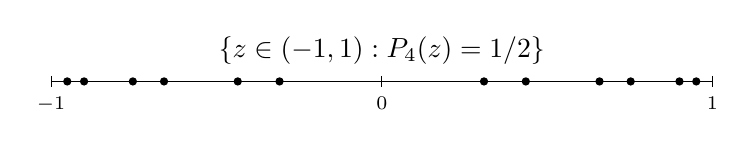
\begin{tikzpicture}[x=4.2cm,y=1cm]
 \draw[semithick] (-1,0)--(1,0);
 \foreach \x in {-1,0,1}{
    \draw (\x,.07)--(\x,-.07) node[below,font=\scriptsize] {\(\x\)};
 }
 \foreach \a in {5,7,11,13,17,19}{
   \pgfmathsetmacro{\xx}{sqrt((1+cos(7.5*\a)/cos(11.25))/2)}
   \fill (\xx,0) circle[radius=1.5pt];
   \fill (-\xx,0) circle[radius=1.5pt];
 }
 \node[above] at (0,.09) {\(\{z\in(-1,1):P_4(z)=1/2\}\)};
\end{tikzpicture}
\caption{The first vertical return block \(P_4=T_8\circ(c_4T_2)\). Top: the critical point \(0\) returns to \(0\) with local order two. Bottom: the regular value \(1/2\) has twelve simple inverse images in \((-1,1)\), giving distinct local inverse charts for the fold.}
\label{fig:fold-block}
\end{figure}


Fix $r\ge 1$ and $R=2^r$. Number complete tuned blocks from the \emph{output} backward with lengths $\ell_i:=i+3$ ($i\ge 1$) and cumulative lengths $b_0:=0$, $b_i:=\sum_{m=1}^i \ell_m = \frac{i(i+7)}{2}$, and let $I:=\max\{i\ge 0 : b_i\le r\}$. Starting from $v=y^2$ and $u_0(y):=2v-1$, define $u_1,\dots,u_r$ by applying $r-b_I$ ordinary $T_2$ maps first, followed by the blocks $P_{\ell_I},P_{\ell_{I-1}},\dots,P_{\ell_1}$. Equivalently, $u_{k+1}=c_k(2u_k^2-1)$ for $0\le k<r$, where $c_k=\cos(\pi/2^{\ell_i})$ at the initial map $k=r-b_i$ of each block $i\in\{1,\dots,I\}$ and $c_k=1$ otherwise. At stage $k$, let $\Phi_k(z)$ denote the remaining $(r-k)$-fold composition sending $z=u_k(y)$ to $u_r(y)=\Phi_k(u_k(y))$.

\begin{lemma}[Branch counts and local flatness orders of recurrent folds]\label{lem:recurrent-folds}
For $0\le k<r$ and $j:=r-k$, set
\begin{equation}\label{eq:ej-Yk}
  e_j := 2^{\max(1,\,\#\{i\ge 1:\, b_i\le j\})}, \qquad
  Y_k := 2^{k+1}\prod_{\substack{1\le i\le I \\ r-b_{i-1}\le k}} \left(1 - \frac{4}{2^{\ell_i}}\right).
\end{equation}
Then:
\begin{enumerate}[label=(\alph*),nosep]
  \item For each $0\le k<r$, $u_k(y)=0$ has at least $Y_k$ simple real roots $y\ne 0$ (where $z=u_k(y)$ is a local diffeomorphism), and the roots selected at distinct stages $k\ne k'$ are automatically disjoint.
  \item For each $0\le k<r$, $\Phi_k(z)$ is an even polynomial with $\Phi_k(0)\in\{-1,0,1\}$ and $\ord_0(\Phi_k-\Phi_k(0))=e_j$; consequently $\Xi(y):=(u_r(y)^3-u_r(y))^2$ satisfies $\Xi=C_k z^{2e_j}(1+O(z^2))$ near $z=u_k(y)=0$ with $C_k>0$ depending only on $k$.
  \item Uniformly for every integer $r\ge 1$,
  \begin{equation}\label{eq:fold-sums}
    \sum_{k=0}^{r-1}\left(1-\frac{Y_k}{2^{k+1}}\right) \le \frac52, \qquad
    \sum_{j=1}^r \frac{1}{e_j} \le 10, \qquad
    \sum_{k=0}^{r-1} 2^{k+1} e_{r-k} < 6R.
  \end{equation}
\end{enumerate}
\end{lemma}

\begin{proof}
First examine preimages of $w\in(-1,1)$ under $P_\ell(z)=T_{b_\ell^*}(c_\ell T_2(z))$. On each of the $b_\ell^*=2^{\ell-1}$ open intervals $(\cos\frac{(m+1)\pi}{b_\ell^*},\cos\frac{m\pi}{b_\ell^*})$ ($0\le m<b_\ell^*$), $T_{b_\ell^*}(t)=w$ has one simple root $t_m$. Discarding the two extreme intervals $m=0$ and $m=b_\ell^*-1$ leaves $b_\ell^*-2$ interior roots satisfying
\[
  |t_m| \le \cos\left(\frac{\pi}{b_\ell^*}\right) < \cos\left(\frac{\pi}{2b_\ell^*}\right) = c_\ell,
\]
so $t_m/c_\ell\in(-1,1)$ and $T_2(z)=t_m/c_\ell$ yields two simple roots $z=\pm\sqrt{(1+t_m/c_\ell)/2}\in(-1,1)\setminus\{0\}$. Thus every $w\in(-1,1)$ has at least $2(b_\ell^*-2)=2^\ell(1-4/2^\ell)$ simple preimages in $(-1,1)$ under $P_\ell$. Moreover, for a proper initial segment of $1\le d<\ell$ maps of $P_\ell$, the composition is $T_{2^{d-1}}(c_\ell T_2(z))$, and every root $\cos\frac{(2m+1)\pi}{2^d}$ of $T_{2^{d-1}}(t)=0$ has modulus $\le\cos\frac{\pi}{2^d}\le\cos\frac{\pi}{2^{\ell-1}}<c_\ell$, giving all $2^d$ simple interior roots of $0$. Tracing $0$ backward from stage $k$ to $u_0=2y^2-1$: a terminal partial tuned block keeps all $2^d$ simple roots in $(-1,1)$; each complete preceding block $P_{\ell_i}$ ($r-b_{i-1}\le k$) multiplies the count of simple interior preimages by at least $2^{\ell_i}(1-4/2^{\ell_i})$; initial ordinary $T_2$ maps double the count in $(-1,1)$; and finally $2y^2-1=w\in(-1,1)$ yields two nonzero opposite real roots $y=\pm\sqrt{(1+w)/2}$. This produces $Y_k$ simple roots of $u_k(y)=0$. If $u_k(y_*)=0$, then $u_{k+1}'(y_*)=4c_k u_k(y_*)u_k'(y_*)=0$ and inductively $u_{k'}'(y_*)=0$ for every $k'>k$, so $y_*$ can never be a simple root of a later $u_{k'}$, proving~(a).

For~(b), $\Phi_k(z)$ begins with $c_k(2z^2-1)$ and is therefore even in $z$. Let $i_0=\#\{i\ge 1 : b_i\le j\}$, so $b_{i_0}\le j < b_{i_0+1}$ (with $b_{I+1}=\infty$). If $i_0=0$ ($1\le j\le 3$), the last $j$ maps of the sequence are the final $j<\ell_1=4$ maps of $P_{\ell_1}$ (or initial $T_2$'s if $I=0$), all of which are ordinary $T_2$'s: the first sends $0\mapsto -1$ with local degree $2$, and any subsequent $T_2$'s send $-1\mapsto 1\mapsto 1$ with local degree $1$, so $\Phi_k(0)\in\{-1,1\}$ and $\ord_0(\Phi_k-\Phi_k(0))=2=e_j$. If $i_0\ge 1$ and $j=b_{i_0}$, then $\Phi_k=P_{\ell_1}\circ\cdots\circ P_{\ell_{i_0}}$ fixes $0$ with local degree $2^{i_0}=e_j$. If $i_0\ge 1$ and $j=b_{i_0}+m$ with $m\ge 1$, the first $m$ maps of $\Phi_k$ are ordinary $T_2$'s (either the trailing $m<\ell_{i_0+1}$ maps of $P_{\ell_{i_0+1}}$ or initial $T_2$'s), which send $0\mapsto w_*\in\{-1,1\}$ with local degree $2$; next $P_{\ell_{i_0}}$ sends $w_*\mapsto 0$ with local degree $1$ (since $P_{\ell_{i_0}}'(\pm 1)\ne 0$); and the remaining $i_0-1$ blocks $P_{\ell_{i_0-1}},\dots,P_{\ell_1}$ fix $0$ with local degree $2^{i_0-1}$, giving $\Phi_k(0)=0$ and local degree $2\cdot 1\cdot 2^{i_0-1}=2^{i_0}=e_j$. Since $t^3-t$ has simple roots at $-1,0,1$, $(\Phi_k(z)^3-\Phi_k(z))^2=C_k z^{2e_j}(1+O(z^2))$ with $C_k>0$.

For~(c), each completed block $i\in\{1,\dots,I\}$ appears in the product for $Y_k$ for at most the $b_{i-1}<b_i$ indices $k\ge r-b_{i-1}$. Using $1-\prod(1-\delta_i)\le\sum\delta_i$ for $\delta_i\in(0,1)$ gives
\[
  \sum_{k=0}^{r-1}\left(1-\frac{Y_k}{2^{k+1}}\right)
  \le \sum_{i=1}^\infty b_{i-1}\frac{4}{2^{i+3}}
  = \sum_{i=2}^\infty \frac{(i-1)(i+6)}{2^{i+2}}
  = \sum_{m=1}^\infty \frac{m(m+7)}{2^{m+3}} = \frac{5}{2}.
\]
Similarly, $e_j=2$ for $1\le j<b_2=9$ ($8$ indices) and $e_j=2^i$ for $b_i\le j<b_{i+1}$ ($\ell_{i+1}=i+4$ indices, $i\ge 2$), whence $\sum_{j=1}^r e_j^{-1}\le \frac{8}{2}+\sum_{i=2}^\infty (i+4)2^{-i}=4+\frac{7}{2}<10$. Finally, because every block has length $\ge 4$, $b_i\ge 4i$, so $\#\{i\ge 1:b_i\le j\}\le j/4$ and $e_j\le 2\cdot 2^{j/4}$; thus $\sum_{k=0}^{r-1}2^{k+1}e_{r-k}=2R\sum_{j=1}^r 2^{-j}e_j\le 4R\sum_{j=1}^\infty 2^{-3j/4}=\frac{4R}{2^{3/4}-1}<6R$.
\end{proof}

The cosine parameters specify real model folds. At the end of the proof of Theorem~\ref{thm:finite-folded}, the area moment has a simple zero in each selected energy interval. These zeros persist under one sufficiently close rational approximation of the expanded polynomials in \(y^2\).


\subsection{Attainable primitives on a full sublevel disk}

A change of the vertical potential moves the boundary of a disk for \(U(x)+V(y)\). To express its effect as an interior derivative we must cancel possible poles on the entire disk. Write \(\PP_n\) for the univariate polynomials of degree at most \(n\), with \(\PP_n=\{0\}\) for \(n<0\). In a row use a smooth coordinate $z=z(y)$ with $z'(y)\ne0$. Let $J(z)$ be any nonconstant polynomial, and set $\bar V(y)=\phi(J(z))$, $\bar F(y)=\psi(J(z))$. Differentiate in the argument of $\phi,\psi$ before composing:
\[
 D_0=\phi'(J(z)),\qquad E_0=\psi'(J(z)),\qquad
 \delta=\deg D_0\ge1,\quad \eta=\deg E_0\ge0 .
\]

\begin{lemma}[Division on a full sublevel disk]
\label{lem:whole-disk-division}Factor $D_0=C D_{\mathrm{reg}}$ with $D_{\mathrm{reg}}$ nonzero on the entire vertical projection of each closed disk in its row coordinate. Write $g=\deg D_{\mathrm{reg}}$, $\Gamma=\gcd(D_{\mathrm{reg}},E_0)$ monic and $\ell=\deg \Gamma$. For $d_B\ge\max(0,\eta-\ell-1)$ and $\deg R\le g+d_B$, the equation
\begin{equation}\label{eq:bezout-rep}
 N_0=C R=D_0B-E_0A,\qquad C\mid A,\quad \deg B\le d_B
\end{equation}
is solvable exactly when $\Gamma\mid R$. The solution normalized by $\deg(A/C)<g-\ell$ is unique (degree $<0$ means the zero polynomial). In particular $\deg A\le\delta-\ell-1$. The attainable numerators $R$ have codimension $\ell$ in $\PP_{g+d_B}$. Rational factorization data and rational $R$ give rational corrections.

Let $\Omega_\lambda(E)$ be bounded components of the strict sublevel set of $U(x)+\bar V(y)+\lambda A(z(y))$ at $E$, with Jordan closures in the row charts and regular boundaries depending smoothly on $(\lambda,E)$ for $|\lambda|$ small and $E$ in a compact bracket. With $\bar F_\lambda=\bar F+\lambda B(z(y))$, one has in $C^1$ of that bracket
\begin{equation}\label{eq:shape-derivative-green}
 \left.\partial_\lambda\right|_0\iint_{\Omega_\lambda(E)}\partial_y\bar F_\lambda\,\dd x\dd y
  =\iint_{\Omega_0(E)}\partial_y\bigl((R/D_{\mathrm{reg}})(z(y))\bigr)\,\dd x\dd y .
\end{equation}
\end{lemma}

\begin{proof}
Put $A=C h$. Canceling $C$ gives $R=D_{\mathrm{reg}} B-E_0 h$, so $\Gamma\mid R$ is necessary in every degree. If $\Gamma\mid R$, reduce modulo $D_{\mathrm{reg}}/\Gamma$: for $g>\ell$ take $h$ to be the residue of $-(R/\Gamma)(E_0/\Gamma)^{-1}$ modulo $D_{\mathrm{reg}}/\Gamma$, and for $g=\ell$ take $h=0$. Then $B=(R+E_0h)/D_{\mathrm{reg}}$ is a polynomial and $\deg(E_0h)\le\eta+g-\ell-1\le g+d_B$ whenever $h\ne0$, which proves existence, uniqueness, and the degree bounds. Multiples of $\Gamma$ of degree at most $g+d_B$ form a subspace of codimension $\ell$, and on the row $A/D_0=h/D_{\mathrm{reg}}$ is smooth throughout the disk.

On a regular boundary collar of $\partial\Omega_0(E)$, $|\nabla(U+\bar{V})|>0$ and the outward unit normal to $\Omega_0(E)$ is $\mathbf{n}=(n_x,n_y)=\nabla(U+\bar{V})/|\nabla(U+\bar{V})|$. Differentiating $U(x)+\bar{V}(y)+\lambda A(z(y))=E$ gives normal boundary velocity $-A(z(y))/|\nabla(U+\bar{V})|$. Since $\partial_y\bar{F}=E_0(z)\partial_y J$ and $\partial_y\bar{V}=D_0(z)\partial_y J$, and since $A/D_0$ is smooth throughout $\overline{\Omega_0(E)}$, the identity $A(z)\partial_y\bar{F}=(A(z)E_0(z)/D_0(z))\partial_y\bar{V}$ holds everywhere by continuity across canceled zeros of $D_0$ and $\partial_y J$. Applying the divergence theorem to $(0,A(z)E_0(z)/D_0(z))$ on the Jordan domain $\Omega_0(E)$ gives
\begin{align*}
  -\oint_{\partial\Omega_0(E)} \frac{A(z(y))\partial_y\bar{F}(y)}{|\nabla(U+\bar{V})|}\dd s
  &= -\oint_{\partial\Omega_0(E)} \frac{A(z(y))E_0(z(y))}{D_0(z(y))}\,n_y\dd s \\
  &= -\iint_{\Omega_0(E)} \partial_y\left(\frac{A(z)E_0(z)}{D_0(z)}\right)\dd x\dd y.
\end{align*}
Adding the interior derivative $\iint_{\Omega_0(E)}\partial_y B(z(y))\dd x\dd y$ yields~\eqref{eq:shape-derivative-green}; smooth level-set coordinates in a compact collar of $\partial\Omega_0(E)$ justify differentiating~\eqref{eq:shape-derivative-green} once with respect to $E$ (critical points of $U+\bar{V}$ strictly inside $\Omega_0(E)$ lie outside the boundary collar and contribute no boundary terms).
\end{proof}

The divisibility test concerns the chosen rational primitive. Two primitives differing by a constant, for instance, give the same energy function. In Theorem~\ref{thm:finite-folded} the inherited derivatives are coprime, so their B\'ezout identity gives \(\Gamma=1\) after composition. Reflection makes the inherited moment vanish on a new row. The proof controls the roots of \(D_0\) before division and uses nested polynomial row coordinates to keep all corrections within the physical degree budget. A single fifth-degree fold illustrates both realizability and an obstruction after changing the inherited drive \cite[Proposition~\othernumber{prop:quintic}{S6.1}]{LuElectronic}.

\begin{lemma}[Continuation of a sublevel disk]\label{lem:disk-core}
Let $H$ be smooth and $a<E_-<E_+<b$. Suppose a closed Jordan disk $K_a$ satisfies $H\le a$ there, $\partial K_a\subset\{H=a\}$, and a compact regular annulus meets $K_a$ exactly in their common boundary $\partial K_a$. Suppose its levels foliate the annulus from $a$ on this inner boundary to $b$ on its outer boundary. For all sufficiently $C^1$-close $\widetilde H$ on their union, each $E\in[E_-,E_+]$ encloses a unique Jordan sublevel component containing $K_a$. Its boundary is regular and, for smooth families of $\widetilde H$, varies smoothly in the parameters and $E$. Moreover, if $K_a$ and $\widetilde H$ are invariant under an involution $R$ of the domain, then this continued sublevel component is also $R$-invariant.
\end{lemma}
\begin{proof}
Using the flow of $\nabla H/|\nabla H|^2$ on the compact annulus, introduce coordinates $(\theta,t)\in S^1\times[a,b]$ in which $H(\theta,t)=t$. Let $g=\min|\nabla H|>0$ on the annulus; whenever $\|\nabla(\widetilde H-H)\|_\infty<g/2$ and $\|\widetilde H-H\|_\infty<\min(E_--a,b-E_+)$, we have $\partial_t\widetilde H>1/2$ across the annulus while the core $K_a$ lies strictly below every level $E\in[E_-,E_+]$ and the outer boundary $t=b$ lies strictly above it. Each radial segment $\theta=\text{const}$ therefore intersects $\widetilde H=E$ in a single point, defining a smooth graph $t=t_E(\theta)$ that varies smoothly with $E$ and with smooth parameters of $\widetilde H$. The core $K_a$ together with the region of the annulus beneath this graph forms the unique regular Jordan sublevel component of $\widetilde H<E$ containing $K_a$, isolated from the exterior by $t=b$ and permitting arbitrary critical points inside $K_a$. If an involution $R$ preserves both $K_a$ and $\widetilde H$, then the image of this component under $R$ is again a connected component of $\{\widetilde H<E\}$ containing $K_a$ and therefore coincides with it. Splitting the area integral over the fixed core and the annulus region $a\le t\le t_E(\theta)$ yields continuity of area moments and their first energy derivatives under smooth perturbations of $\widetilde H$.
\end{proof}



\section{Realizing the finite sum in one polynomial field}\label{sec:joint-proof}

\subsection{A division argument on each full oval disk}

Fix $r\ge 1$, $R=2^r$, an even integer $a\ge 2$, integers $p\ge 6aR$ and $d\ge 6R$, a power of two $q_{\max}\ge 2$, an even integer $s\ge 2$, and $X_*:=q_{\max} s$. For each $j\in\{1,\dots,r\}$, choose a dyadic group size $q_j\in\{2,4,\dots,q_{\max}\}$ dividing $q_{\max}$, and for $0\le k<r$ with $j=r-k$ put
\begin{equation}\label{eq:folded-stage-modes}
  \alpha_k := a e_j, \qquad
  M_k := \left\lfloor\frac{p}{2^{k+1}}\right\rfloor + \left\lfloor\frac{d+2^k}{2^{k+1}}\right\rfloor, \qquad
  L_k := \pos{M_k - \alpha_k},
\end{equation}
where $e_j$ and $Y_k$ are given by Lemma~\ref{lem:recurrent-folds}. In the sum below \(Y_k\) counts disjoint vertical row charts. Each row contains \(X_*/q_{r-k}\) horizontal clusters. The factor \(B_{q_{r-k},\alpha_k}(L_k)\) counts the simple-zero brackets obtained in each cluster. The selected collars must persist for one choice of the physical coefficients.
\begin{theorem}[Finite joint-budget theorem]\label{thm:finite-folded}
Under the above assumptions, there exists a polynomial vector field $X=(P,Q)\in\Q[x,y]^2$ with coprime components of the form~\eqref{eq:separable-template} with $V,F\in\Q[y^2]$, $F(0)=0$, satisfying
\begin{gather}
  |\supp P| = p,\quad |\supp Q| = X_*+d, \qquad
  D(X) = \max(2p-1,\,2X_*-1,\,2d), \label{eq:finite-ledger} \\
  \#\{\text{hyperbolic limit cycles of } X\} \ge \sum_{k=0}^{r-1} Y_k\,\frac{X_*}{q_{r-k}}\,B_{q_{r-k},\alpha_k}(L_k). \label{eq:finite-cert}
\end{gather}
Moreover, each length $L_k$ in~\eqref{eq:finite-cert} may independently be replaced by any integer $0\le l_k\le L_k$.
\end{theorem}

The proof follows the two inputs in the first line of the diagram through to a common return parameter in the last. Each arrow concerns one fixed finite allocation.
\[
\begin{gathered}
 \underbrace{\text{endpoint expansions}\ \longrightarrow\
   \text{brackets on shared wells}}_{\text{Lemmas \ref{lem:saddle-singular}--\ref{lem:horizontal-glue}}}
 \quad+\quad
 \underbrace{\text{real rows and their orders}}_{\text{Lemma \ref{lem:recurrent-folds}}}
 \\[-1pt]
 \Downarrow\quad\text{continued disks and strict signs (Lemma \ref{lem:disk-core})}\\
 \text{separated roots on each row}\ \longrightarrow\
 \text{division on its disks (Lemma \ref{lem:whole-disk-division})}\\
 \Downarrow\quad\text{corrections in descending order of the stages}\\
 \text{open set of physical coefficients}\ \longrightarrow\
 \text{one rational field (Lemma \ref{lem:hyperbolic-return}).}
\end{gathered}
\]
\begin{proof}
\emph{Model brackets.}
Write $p_i=\lfloor p/2^i\rfloor$ and $d_i=\lfloor d/2^i\rfloor$. Apply Lemma~\ref{lem:horizontal-glue} to the list of triples $(q_{r-k},\alpha_k,l_k)$ ($0\le k<r$, omitting stages for which $B_{q_{r-k},\alpha_k}(l_k)=0$), obtaining one even rational polynomial $W\in\Q[x]$ of degree $2X_*$, rational odd primitives $S_k(Z)$ of degree at most $2l_k-1$, and at least $(X_*/q_{r-k})B_{q_{r-k},\alpha_k}(l_k)$ disjoint compact simple-zero brackets for $\iint S_k'(Z)\dd x\dd Z$ on the model $W(x)+Z^{2\alpha_k}$ at each active stage $k$. For each compact model bracket extend its energy interval slightly at each end within the same branch of regular ovals. In $W(x)+Z^{2\alpha_k}$ the lower extended oval bounds a closed disk on which the energy is at most its boundary value, by the sublevel description in Section~\ref{sec:horizontal}. The shell up to the upper extended oval is a regular annulus. For an outgoing bracket the lower extension lies above the enclosed saddle heights. These disks and annuli supply the cores and margins of Lemma~\ref{lem:disk-core} in each rescaled chart.

The division on a new row is with respect to \(J=c_k(2z^2-1)\). Here \(\Xi\) vanishes to order \(2e\) in \(z\), so the \(J\)-derivative of \(\Xi^a\) alone would vanish to order \(2ae-2\). A positive linear term in \(\Xi\) reduces this order to \(2e-2\). After that factor is removed the divisor must stay nonzero on the entire disk, while the chosen regular energy brackets must persist. The following scale gives both properties. Using \(\Xi=(u_r^3-u_r)^2\) from Lemma~\ref{lem:recurrent-folds}(b), set
\[
  U(x) := \rho W(x), \qquad V_* := \Xi^a + \kappa \Xi, \qquad
  \kappa := \kappa_0 \rho^{1-1/a}, \qquad
  \tau_k := \left(\frac{\rho^{1/a}}{C_k}\right)^{1/(2e)}, \quad e := e_{r-k}.
\]
In the rescaled local row coordinate $z=u_k(y)=\tau_k Z$ around any of the $Y_k$ simple roots of $u_k(y)=0$, Lemma~\ref{lem:recurrent-folds}(b) gives $V_*/\rho \to Z^{2ae}+\kappa_0 Z^{2e}$ in $C^2$ on fixed compact $Z$-intervals as $\rho\downarrow 0$. By Lemma~\ref{lem:disk-core} choose a small $\kappa_0>0$ so that every model bracket of $W(x)+Z^{2\alpha_k}$ continues smoothly with strict opposite signs and nonzero $E$-slope to $W(x)+Z^{2ae}+\kappa_0 Z^{2e}$. The selected roots at distinct stages are disjoint by Lemma~\ref{lem:recurrent-folds}(a). Across the selected rows at all stages (a total of $\sum_{k=0}^{r-1}Y_k$), choose mutually disjoint $y$-intervals on which $z=u_k(y)$ is a chart and choose their widths before choosing $\rho$. Indeed $\Xi=C_k z^{2e}(1+O(z^2))$ is analytic in $z^2$ with $C_k>0$, hence $\partial_{z^2}\Xi=e C_k z^{2e-2}(1+O(z^2))>0$ on sufficiently small punctured intervals. For all sufficiently small $\rho$ the extended disks fit in the interiors of these intervals.

At stage $k$, view $V_*$ as a polynomial in $J=u_{k+1}=c_k(2z^2-1)$ and let $D_*(z)=\partial_J V_*=(4c_k z)^{-1}\partial_z V_* = (2c_k)^{-1}(a\Xi^{a-1}+\kappa)\partial_{z^2}\Xi$. On the chosen compact row interval in $z$, $D_*(z)$ vanishes at $z=0$ to exact order $2e-2$ and has no other real zeros; dividing out $z^{2e-2}$ yields
\begin{equation}\label{eq:Dstar-limit}
  \frac{D_*(\tau_k Z)}{(\tau_k Z)^{2e-2}}
  = C_*\bigl\{a Z^{2(a-1)e} + \kappa_0 + O_{C^2}(\tau_k^2)\bigr\}, \qquad
  C_* := \frac{e\rho}{2c_k\tau_k^{2e}} > 0.
\end{equation}
Define $\widehat{R}_k(z):=C_*\{a(z/\tau_k)^{2(a-1)e}+\kappa_0\}S_k(z/\tau_k)$ (or $0$ if stage $k$ is skipped). At $V_*$, dividing this polynomial by $D_*/z^{2e-2}$ gives a primitive converging to $S_k$ in $C^2(Z)$ on each fixed compact interval, by \eqref{eq:Dstar-limit} and $\kappa_0>0$. In the rescaled charts $(U+V_*)/\rho$ converges with all derivatives on the extended disks. Lemma~\ref{lem:disk-core} transfers each whole disk there from the model with $\kappa_0 Z^{2e}$. Choose one positive rational $\rho$ small enough for these disks to fit in their row charts and for all compensated moments at $V_*$ to have the strict model signs and slopes, up to the chart orientation.

\emph{A common neighborhood for the disks.} Viewing $D_*$ as a polynomial in $w=z^2$, fix a small complex circle $|w|=r_k$ enclosing $w=0$ and no other complex root of $D_*$. The circle is chosen after fixing $\rho$ and may depend on it. 
For $0\le i\le r$ put $\mathcal E_i^p=\{q(u_i):\deg q\le p_i\}\subset\PP_p(v)$, where $v=y^2$. Then $\mathcal E_{i+1}^p\subset\mathcal E_i^p$ since $u_{i+1}=c_i(2u_i^2-1)$ and $2p_{i+1}\le p_i$. At stage $k$ restrict the inherited potential to $\mathcal E_{k+1}^p$. On this subspace recovering the coefficients of $\phi$ from $\bar V=\phi(u_{k+1})$ is a continuous linear operation. Thus $D_0=\phi'(J)$ is a polynomial in $w$ depending continuously on $\bar V$. By Rouch\'e's theorem it has $e-1$ roots in the circle, counted with multiplicity, for all $\bar V$ sufficiently close to $V_*$ in this subspace. Their monic product $C_{\bar V}(w)$ is real and converges to $w^{e-1}$ (equivalently use the contour integrals of the power sums). Polynomial division by this monic factor is continuous even if the degree of $D_0$ increases. Hence $D_{\mathrm{reg}}=D_0/C_{\bar V}(z^2)$ converges with its derivatives to $D_*/z^{2e-2}$ and is bounded away from zero on the fixed row intervals.

For this fixed $\rho$, a sufficiently small perturbation of $\bar V$ within $\mathcal E_{k+1}^p$ preserves the full disks by the same lemma and preserves this primitive estimate by continuity of the quotient. The integral in the physical chart acquires only the fixed orientation sign, since $\partial_y\Upsilon(z(y))\,\dd y$ integrates along vertical slices to the difference of endpoint values of $\Upsilon$. All model endpoint signs and derivative margins therefore persist, with physical energy $\rho E$.

These conditions hold in a relatively open neighborhood $O_k$ of $V_*$ in $\mathcal E_{k+1}^p$. Choose an ambient open $G_k\subset\PP_p(v)$ with $G_k\cap\mathcal E_{k+1}^p=O_k$ and put $\mathcal U_*=\bigcap_{k=0}^{r-1}G_k$. At step $k$ the division conditions apply to $\bar V_{k+1}\in\mathcal U_*\cap\mathcal E_{k+1}^p$. Previously obtained simple brackets give additional open conditions on the pair of physical coefficients. For each fixed allocation there are only finitely many such open conditions.

\emph{Descending corrections.} Since $\deg_{u_r} V_* = 6a \le \lfloor p/2^r\rfloor = p_r$ and $d_r\ge 6$, start at $k=r$ with a pair $(\bar{V}_r,\bar{F}_r)=(\phi_r(u_r),\psi_r(u_r))$ with $\bar{V}_r\in\mathcal{U}_*$, $\bar{F}_r$ arbitrarily close to $0$, exact degrees $\deg_{u_r}\phi_r=p_r$, $\deg_{u_r}\psi_r=d_r$, and $\gcd(\phi_r',\psi_r')=1$ (nonvanishing of the leading coefficients and resultant is open and dense in $\PP_{p_r}\times\PP_{d_r}$). Inductively for $k=r-1,r-2,\dots,0$, given $(\bar{V}_{k+1},\bar{F}_{k+1})=(\phi_{k+1}(u_{k+1}),\psi_{k+1}(u_{k+1}))$ realizing all simple-zero brackets of stages $k'>k$:
\begin{enumerate}[label=\arabic*.,nosep]
  \item Because $\bar{V}_{k+1}$ and $\bar{F}_{k+1}$ are polynomials in $J=c_k(2z^2-1)$, both are \emph{even} in $z=u_k(y)$. Reflection $z\mapsto -z$ leaves each continued regular oval disk $\Omega_{\bar{V}_{k+1}}(E)$ at stage $k$ invariant (the trapping disk and the continued component in the $(x,z)$ chart are reflection invariant). On a vertical slice, $\partial_y\bar F_{k+1}\,\dd y=\dd\bar F_{k+1}$, so each interval $[z_1,z_2]$ in $z$ contributes $\bar F_{k+1}(z_2)-\bar F_{k+1}(z_1)$ up to the fixed orientation of the row chart; the reflected interval contributes its negative, and a symmetric interval contributes zero. Thus $\iint_{\Omega_{\bar{V}_{k+1}}(E)}\partial_y\bar{F}_{k+1}\dd x\dd y=0$ identically on all stage-$k$ collars.
  \item Set $N_0(z):=C_{\bar{V}_{k+1}}(z^2)\widehat{R}_k(z)$. For $1\le l_k\le L_k$, by~\eqref{eq:folded-stage-modes} its degree in $z$ satisfies
  \begin{align*}
    \deg_z N_0 &\le (2e-2) + 2(a-1)e + (2L_k-1) \\
    &= 2\alpha_k + 2L_k - 3 \le 2M_k - 3
     = 2p_{k+1} + 2\left\lfloor\frac{d_k+1}{2}\right\rfloor - 3 \le 2p_{k+1} - 2 + d_k.
  \end{align*}
  Writing $d=2^kd_k+t$ with $0\le t<2^k$ gives $\lfloor(d+2^k)/2^{k+1}\rfloor=\lfloor(d_k+1)/2\rfloor$. Since the inherited derivatives $\phi_{k+1}',\psi_{k+1}'$ are coprime, composing their B\'ezout identity with $J$ gives $\gcd(D_0,E_0)=1$, hence $\Gamma=1$ and $\ell=0$. Here $\delta=2p_{k+1}-2$, $\eta=2d_{k+1}-2$, with $\delta-1\le p_k$ and $d_B:=d_k\ge2d_{k+1}>\eta-1$. Lemma~\ref{lem:whole-disk-division} supplies $B\in\PP_{d_k}(z)$ and $A\in\PP_{p_k}(z)$ with $N_0=D_0 B - E_0 A$ and $C_{\bar{V}_{k+1}}(z^2)\mid A$, so $A/D_0=A/(C_{\bar{V}_{k+1}}D_{\mathrm{reg}})$ is smooth throughout the row and $N_0/D_0=\widehat{R}_k/D_{\mathrm{reg}}$.
  \item By~\eqref{eq:shape-derivative-green}, as $\lambda_k\downarrow 0$, $\lambda_k^{-1}\iint_{\Omega_\lambda(E)}\partial_y(\bar{F}_{k+1}+\lambda_k B(u_k))\dd x\dd y$ converges in $C^1(E)$ on every stage-$k$ collar to $\iint\partial_y(\widehat{R}_k(u_k)/D_{\mathrm{reg}}(u_k))\dd x\dd y$, which has all $Y_k(X_*/q_{r-k})B_{q_{r-k},\alpha_k}(l_k)$ simple-zero brackets. Choose $\lambda_k>0$ small enough to realize these brackets while keeping $\bar{V}_{k+1}+\lambda_k A(u_k)\in\mathcal{U}_*$ and preserving all simple-zero brackets already fixed at stages $k'>k$. If $B_{q_{r-k},\alpha_k}(l_k)=0$ take $A=B=0$ and omit the bracket test. If $k>0$, perturb the resulting pair inside the same open conditions, arbitrarily slightly within $\PP_{p_k}(u_k)\times\PP_{d_k}(u_k)$ to achieve exact degrees $p_k,d_k$ and coprime derivatives in $u_k$ for the next step.
\end{enumerate}

\emph{Passage to a rational field.} At $k=0$, $u_0=2v-1$, so $(\bar{V}_0,\bar{F}_0)\in\PP_p(v)\times\PP_d(v)$ simultaneously realizes every selected simple-zero bracket across all $r$ stages. Because this finite set of regular simple-zero brackets is open in $\PP_p(v)\times\PP_d(v)$ in the physical variable $v=y^2$ (no further fold symmetry is needed after $k=0$), approximate $(\bar{V}_0,\bar{F}_0-\bar{F}_0(0))$ by $(V,F)\in\Q[v]^2$ with $F(0)=0$ so that all $p$ coefficients $[v^i]V$ ($1\le i\le p$) and all $d$ coefficients $[v^j]F$ ($1\le j\le d$) are nonzero rationals. Applying Lemma~\ref{lem:hyperbolic-return} with one small positive rational $\mu\in\Q$ produces~\eqref{eq:finite-cert} simultaneous hyperbolic limit cycles in $X=(V'(y),-U'(x)+\mu F(y))\in\Q[x,y]^2$. Here $\supp P=\{(0,2i-1):1\le i\le p\}$ ($p$ terms), $\supp Q=\{(2l-1,0):1\le l\le X_*\}\sqcup\{(0,2j):1\le j\le d\}$ ($X_*+d$ terms, by Lemma~\ref{lem:horizontal-glue}(b)), giving~\eqref{eq:finite-ledger}; since $P$ depends only on $y$ and $Q$ has nonzero constant leading $x^{2X_*-1}$ coefficient, $\gcd(P,Q)=1$.
\end{proof}

